\documentclass[a4paper,12pt]{article}
\usepackage[polish]{babel}
\usepackage[utf8]{inputenc}
\usepackage{amsfonts}
\usepackage{indentfirst}
\usepackage[T1]{fontenc}
\usepackage{amsmath}
\usepackage{hyperref}
\usepackage{graphicx}
\usepackage{subfig}
\usepackage{fancyvrb}

\textwidth\paperwidth
\advance\textwidth -45mm
\oddsidemargin 18mm
\advance\oddsidemargin -18mm
\evensidemargin 18mm
\advance\evensidemargin -18mm
\topmargin -30mm
\advance\topmargin 17mm
\setlength\textheight{45\baselineskip}
\addtolength\textheight{\topskip}
\marginparwidth 15mm


\title{
Zaawansowane metody uczenia maszynowego \\
Projekt 1
}
\author{
Mikołaj Małkiński \\
\texttt{malkinskim@student.mini.pw.edu.pl}
}
\date{20 Apr 2019}

\begin{document}
    \maketitle

    \section{Wstęp}
    %TODO write me

    \section{Przygotowanie danych}

    \subsection{Brakujące dane}
    %TODO add wykres
    Zbiór danych zawiera wiele kolumn które nie są w pełni wypełnione danymi.
    Analiza wykazała, że tylko 20 kolumn posiadały wszystkie wartości.
    Wykres~\ref{fig:missing-data} przedstawia zależność między stopniem braku danych a liczbą kolumn.
    Istnieje kilka możliwych podejść które można zastosować w tym przypadku.
    Po pierwsze, można kompletnie zignorować i wybrać model który jest w stanie sam odpowiednio obsłużyć luki w zbiorze.
    Przykładem takiego modelu jest \textit{XGBoost}.
    Jednakże, nie wszystkie algorytmy do klasyfikacji są przygotowane na braki w danych,
    Dlatego, aby móc porównać działanie kilku modeli na tym samym zbiorze podjęto decyzję o wypełnieniu brakujących danych.

    \begin{figure}[!h]
        \centering
        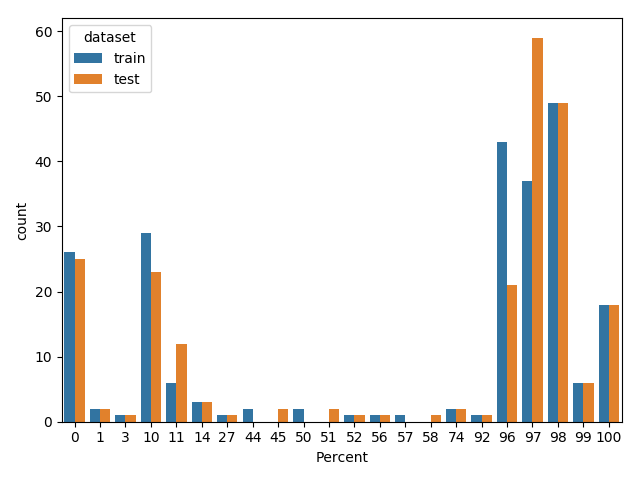
\includegraphics[width=\textwidth]{../doc/images/missing-data.png}
        \caption{Brakujące dane}
        \label{fig:missing-data}
    \end{figure}

    Niektóre z kolumn posiadały nawet ponad 90\% brakująych danych.
    Nie mając żadnych informacji o zbiorze danych oraz nie wiedząc co dana kolumna reprezentuje, ciężko stwierdzić z czego wynika taki duży brak.
    Może to oznaczać zwyczajnie brak pomiaru, wartość ważną równie dobrze jak ta która istnieje w danej kolumnie lub w danym przypadku wartość w tej kolumnie może nie mieć żadnego znaczenia dla konkretnego wiersza.
    Ze względu na duży rozmiar zbioru danych, podjęto decyzję o kompletnym usunięciu części z takich kolumn, które mają więcej braków niż dany procent.
    Resztę poddano imputacji.

    Kolumny w zbiorze można podzielić na 2 rodzaje: \textit{numeryczne} i \textit{kategoryczne}.
    Aby wypełnić pierwszy z nich, brakujące dane w każdej kolumnie wypełniono jej medianą.
    Oczywiście w innych przypadkach mogłyby zostać także inne funkcje, takie jak średnia lub moda.
    W przypadku kolumn kategorycznych, dodano nową kategorię: \textit{unknown}, która wypełniła braki w tych kolumnach.

    \subsection{Unikalność danych}
    Następnie, analizie poddano liczbę unikalnych wartości dla każdej z kolumn.
    Zbiór zawierał kolumny wypełnione tylko jedną tą samą wartością.
    Takie kolumny nie niosą ze sobą żadnej wartości więc zostały one usunięte
    Dodatkowo, część kolumn kategorycznych, posiadały bardzo dużo unikalnych wartości.
    Można przypuszczać że są to dane tekstowe, któ©e także nie przyniosą pozytywnych efektów w klasyfikacji.
    Te kolumny zostały także usunięte.

    \subsection{Kolumny kategoryczne}
    Niektóre algorytmy klasyfikacji wymagają aby zbiory na których zostaną użyte posiadały tylko cechy numeryczne.
    Z tego powodu, cechy kategoryczne musiały zostać przekształcone w liczbowe.
    Najprostszym sposobem jest zamienienie każdej z kategorii na unikalną liczbę.
    Jednakże to implikuje pewien porządek w tej kolumnie, który tak na prawdę nie występuje.
    Dlatego każdą kolumnę przekształcono w \textit{n} nowych kolumn, gdzie \textit{n} to liczba kategorii dla danej kolumny.
    Proces ten nazywany jest \textit{One-hot encoding}.

    \section{Klasyfikacja}

    \subsection{Użyte modele}

    \subsection{Wybrany model}

    \section{Podsumowanie}

    \subsection{Wyniki}

    \subsection{Możliwe ulepszenia}

    \bibliographystyle{plain}
    \bibliography{report.bib}

\end{document}
